\documentclass[12pt]{article}
\usepackage{graphicx}
\usepackage{fixltx2e}
\graphicspath{ {/figs} }
\makeatletter% Set distance from top of page to first float
\setlength{\@fptop}{2pt}
\makeatother
%
% Title.
\title{\textbf{Experiment 1: Characterization of a CMOS Inverter}}
% Author
\author{\textit{Bhishma Dedhia -- 16D170005}}

% begin the document.
\begin{document}

% make a title page.
\maketitle

% section 1: overview.
\section{Overview}

The CMOS inverter is the simplest static complementary CMOS logic gate.
It is also representative of all static complementary logic gates, in the sense
that the qualitative behaviour of an arbitrary static complementary gate is
captured by that of the inverter. In this experiment we aim to:
\begin{itemize}
\item Measure the transfer characteristic of the CMOS inverter.
\item Observe the output characteristic of the inverter.
\item Measure the delay characteristics.
\item Observe the effect of Input voltage on delay.
\item Measure the current drawn from the power supply.
\end{itemize}

% section 2: setup/approach.
\section{Experimental Setup}
The components required are:
\begin{itemize}
\item IC MM74C04 - 4
\item Breadboard.
\item Decoupling capacitors -0.1 µF.
\item 1 ohm Resistor for switching current.
\item 1.2 Kohm Resistor for output characteristics.
\item 20 Kohm potentiometer for output characteristics.
\item Opamp as buffer - TL072.
\item Connecting wires, voltmeter, Ammeter
\end{itemize}
The IC MM74C404 is used as the elementary CMOS unit. It is used to measure the Transfer and output characteristics. A 17 unit oscillator is constructed to measure the Delay characteristics and the Supply power effect on delay. Further the ring oscillator is modified to measure the current drawn. In section 3, I have given the detailed setup used for each part along with the answers to the assignment.  
\section{Observations}
\subsection{DC Transfer Characteristics}
This experiment helps us to find the input vs output behavior of the CMOS inverter. We can also find the V\textsubscript{sw} the switching Voltage of the CMOS. The circuit layout is:
\begin{figure}[h]
    \centering
    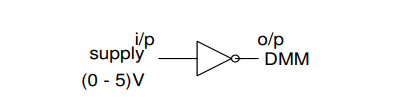
\includegraphics{figs/DC_chts.png}
    \caption{Cicuit Layout}
    \label{fig:my_label}
\end{figure}
\newline The observed values can be found in Table 1. It can be observed that the output voltage falls to zero as the input voltage rises.The switching Voltage V\textsubscript{sw} can be approximated to \textbf{2.46 V}
\newline Table 1 can be better visualized in a plot of the input voltage vs the output voltage. The plot can be found in Figure 2
\begin{figure}[!h]
    \centering
    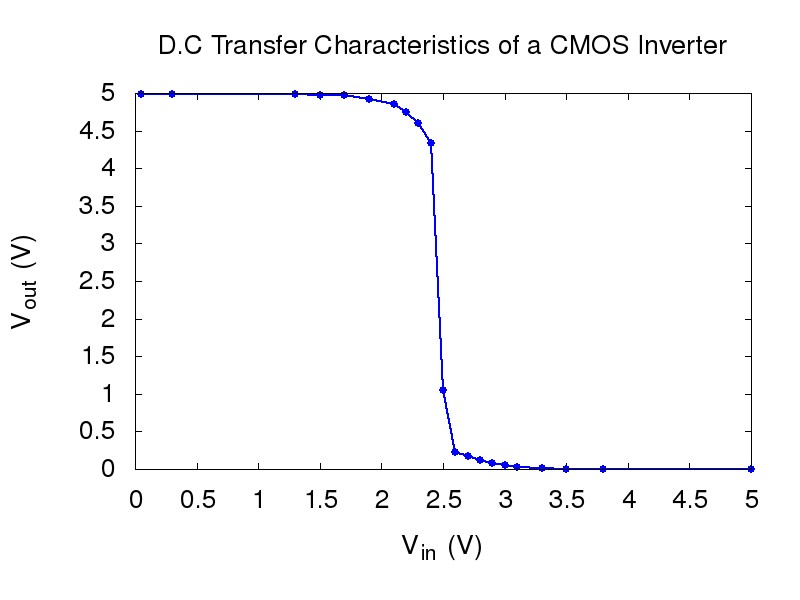
\includegraphics[scale = .6]{figs/DC_ch.jpg}
    \caption{V\textsubscript{out} vs V\textsubscript{in}}
    \label{fig:my_label}
\end{figure}
\begin{table}[h]
\centering  % table will be centered.                                                                                                                                                              
\begin{tabular}{|c | c |}                                                             
\hline  % horizontal line spanning the columns.                                                                                                                                                                    
V\textsubscript{in} (V) & V\textsubscript{out} (V) \\  % table entry 1, separated by &, ended by \\                                                                                                                                                      
\hline  % horizontal line spanning the columns.                                                                                                                                                                    
0.05 & 4.99 \\
0.3	& 4.99 \\
1.3	& 4.99 \\
1.5	& 4.98\\
1.7 & 4.97\\
1.9 & 4.92 \\
2.1 & 4.85\\
2.2 &	4.75\\
2.3	& 4.6\\
2.4	& 4.34\\
2.5	& 1.05\\
2.6	& 0.225\\
2.7	& 0.167\\
2.8	& 0.114\\
2.9	& 0.078\\
3	& 0.056\\
3.1	& 0.03\\
3.3	& 0.008\\
3.5	& 0.002\\
3.8	 & 0.001\\
5 &	0\\
\hline  % horizontal line.                                                                                                                                                                                         
\end{tabular}
\caption{DC Characteristics of the CMOS Inverter}
\label{table:demotable}
\end{table}
\clearpage
\subsection{Output characteristic of a CMOS Inverter}
The output characteristics give us information about the current sourcing/sinking
capability of the inverter. We find how the output voltage varies with
the current drawn from or sunk into the inverter. Note that when the output
of the inverter is high, the output voltage will fall as the current drawn from
the inverter increases. When the output of the inverter is low, the output
voltage will rise as the current sunk by the inverter increases.
The experimental setup isshown in Figure 3.
\begin{figure}[h]
    \centering
    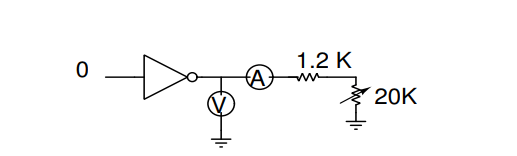
\includegraphics{figs/inputlow.png}
    \caption{Output characteristics when output is high}

    \label{fig:my_label}
\end{figure} 
The setup for low output is similar except that input is 5V and the resistors are connected to V\textsubscript{DD}. We can see  output characteristics when output is high and low in Figure 4 and Figure 5 respectively.The readings of the experiment can be found in Table 2 and Table 3.
\begin{figure}[t]
    \centering
    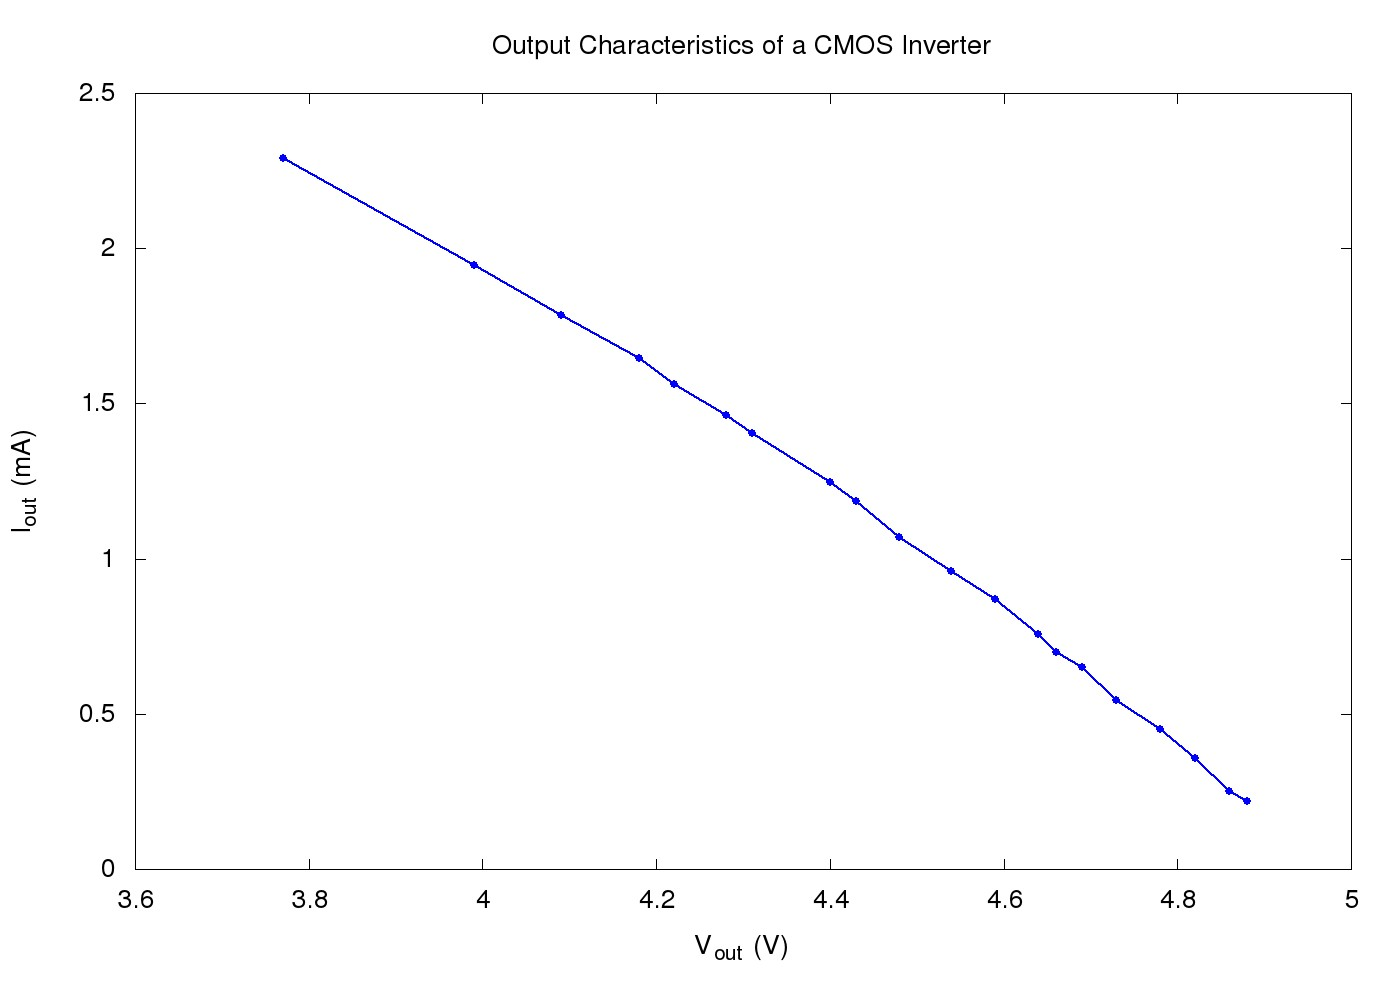
\includegraphics[scale = .40]{figs/When_input_zero.jpg}
    \caption{Output characteristics when output is high}
    \label{fig:my_label}
\end{figure}


   
  

\begin{table}[t]
\centering  % table will be centered.                                                                                                                                                              
\begin{tabular}{|c | c |}                                                             
\hline  % horizontal line spanning the columns.                                                                                                                                                                    
V\textsubscript{out} (V) & I\textsubscript{out} (mA) \\  % table entry 1, separated by &, ended by \\                                                                                                                                                      
\hline  % horizontal line spanning the columns.                                                                                                                                                                   
4.88 &	0.219\\
4.86 &	0.251\\
4.82 &	0.356\\
4.78 &	0.452\\
4.73 &	0.544\\
4.69 &	0.65\\
4.66 &	0.7\\
4.64 &	0.757\\
4.59 &	0.869\\
4.54 &	0.961\\
4.48 &	1.07\\
4.43 &	1.187\\
4.4	  &   1.246\\
4.31 &	1.406\\
4.28 &	1.463\\
4.22 &	1.563\\
4.18 &	1.647\\
4.09 &	1.784\\
3.99 &	1.945\\
3.77 &	2.29\\


\hline  % horizontal line.                                                                                                                                                                                         
\end{tabular}
\caption{Output characteristics when output is high}
\label{table:demotable}
\end{table}



\begin{figure}[t]
    \centering
    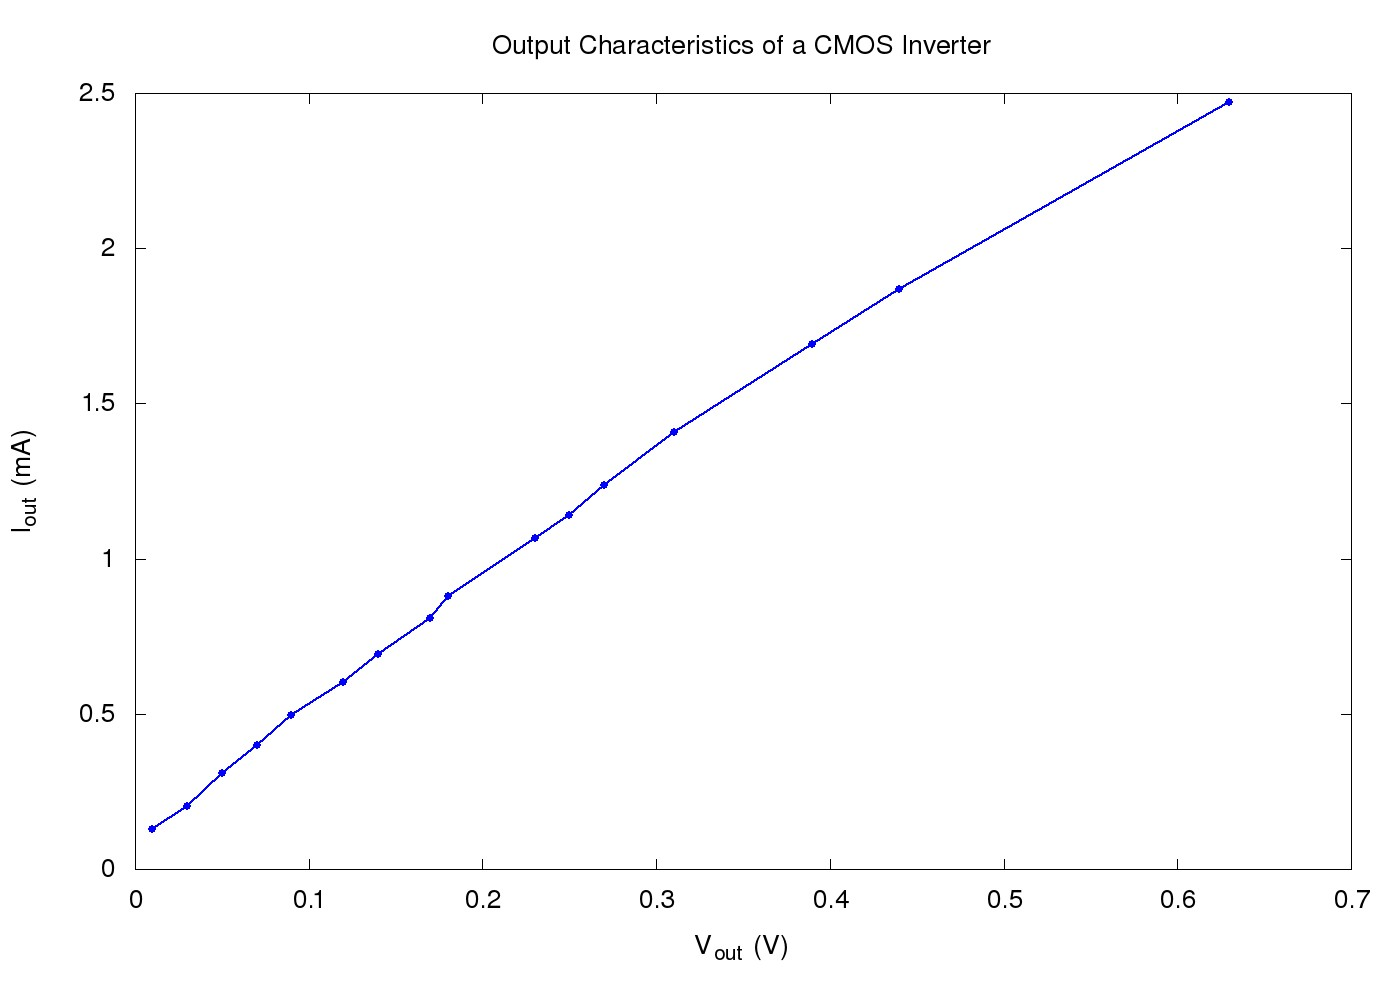
\includegraphics[scale = .40]{figs/When_input_High.jpg}
    \caption{Output characteristics when output is low}
    \label{fig:my_label}
\end{figure}

 
 \begin{table}[!t]
\centering  % table will be centered.                                                                                                                                                              
\begin{tabular}{|c | c |}                                                             
\hline  % horizontal line spanning the columns.                                                                                                                                                                    
V\textsubscript{out} (V) & I\textsubscript{out} (mA) \\  % table entry 1, separated by &, ended by \\                                                                                                                                                      
\hline  % horizontal line spanning the columns.                                                                                                                                                                   
0.01 &	0.128\\
0.03 &	0.203\\
0.05 &	0.309\\
0.07 &	0.398\\
0.09 &	0.496\\
0.12 &	0.601\\
0.14 &	0.694\\
0.17 &	0.81\\
0.18 &	0.88\\
0.23 &	1.066\\
0.25 &	1.14\\
0.27 &	1.236\\
0.31 &	1.408\\
0.39 &	1.69\\
0.44  &	1.867\\
0.63 &	2.47\\

\hline  % horizontal line.                                                                                                                                                                                         
\end{tabular}
\caption{Output characteristics when output is low}
\label{table:demotable}
\end{table}
\clearpage
\subsection{ Delay Characterization of the inverter}
An inverter produces delay in digital circuits and is an important factor. We have tried to measure the delay using a 17-Ring oscillator. The delay can be modelled as:
\[d_{abs} = k_{0} + k_{1}C_{load}\]
This can be expressed in multiples of $\tau$ as:
\[d_{inv} = p_{inv} + h\]
 For 17 oscillator ring :
 
 Oscillation period =  $\tau$ \times(34 p\textsubscript{inv} + ( 32 + ( 2 \times ( 1 + \textit{AdditionalLoadOutput})))
 
 The plot of Oscillation Period vs Load is shown in Figure 6. Values can be found in Table 4.
 \begin{figure}[h]
     \centering
     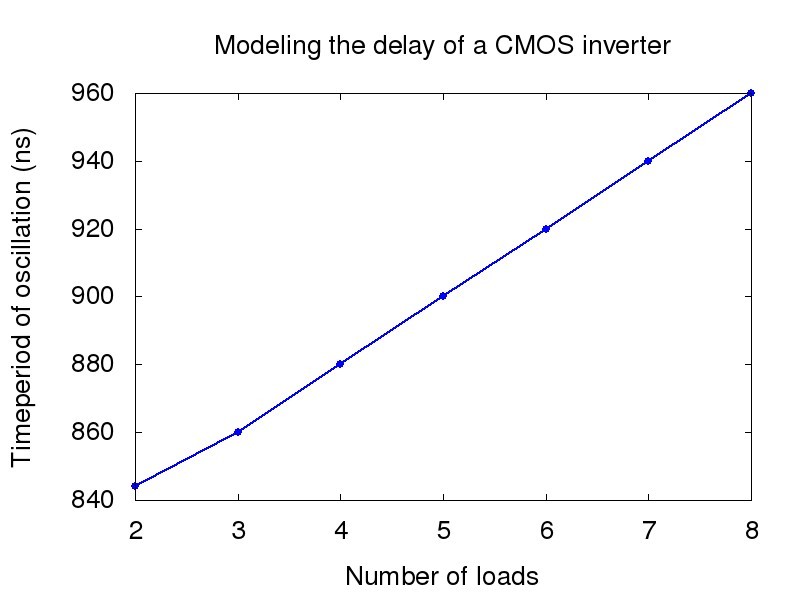
\includegraphics[scale = 0.6]{figs/timeperiods.jpg}
     \caption{Delay Characterization of inverter}
     \label{fig:my_label}
 \end{figure}
  
 \begin{table}[!h]
\centering  % table will be centered.                                                                                                                                                              
\begin{tabular}{|c | c |}                                                             
\hline  % horizontal line spanning the columns.                                                                                                                                                                    
Number of Loads & Time period of Oscillation (ns) \\  % table entry 1, separated by &, ended by \\                                                                                                                                                      
\hline  % horizontal line spanning the columns.                                                                                                                                                                   
2	& 844\\
3	& 860\\
4	& 880\\
5	& 900\\
6	& 920\\
7	& 940\\
8	& 960\\


\hline  % horizontal line.                                                                                                                                                                                         
\end{tabular}
\caption{Modeling the Delay}
\label{table:demotable}
\end{table}
Slope = 2$\tau$ = 20ns\\
Intercept = $\tau$\times(34p\textsubscript{inv} + 36) = 844

\vspace{20mm}
Hence \textbf{$\tau$} = 10 ns and \textbf{p\textsubscript{inv}} = 1.42

\subsection{Delay Variation with supply voltage}
In digital devices the delay depends on the supply voltage. Hence we vary the input voltage to find its effect on oscillation period. 
\[Delay\propto\frac{V_{DD}}{(V_{DD}-V_{t})^2}\]
This can be validated from the observations. Figure 7 clearly shows the effect.
\begin{table}[!h]
\centering  % table will be centered.                                                                                                                                                              
\begin{tabular}{|c | c |}                                                             
\hline  % horizontal line spanning the columns.                                                                                                                                                                    
Supply Voltage (V) & Time period of Oscillation (us) \\  % table entry 1, separated by &, ended by \\                                                                                                                                                      
\hline  % horizontal line spanning the columns.                                                             

3 &	2.288\\
3.5 &	1.486\\
4	 & 1.152\\
4.5	& 0.937\\
5	& 0.79\\
5.5	& 0.707\\
6	& 0.635\\



\hline  % horizontal line.                                                                                                                                                                                         
\end{tabular}
\caption{Delay variation with supply voltage}
\label{table:demotable}
\end{table}
\begin{figure}[!t]
    \centering
    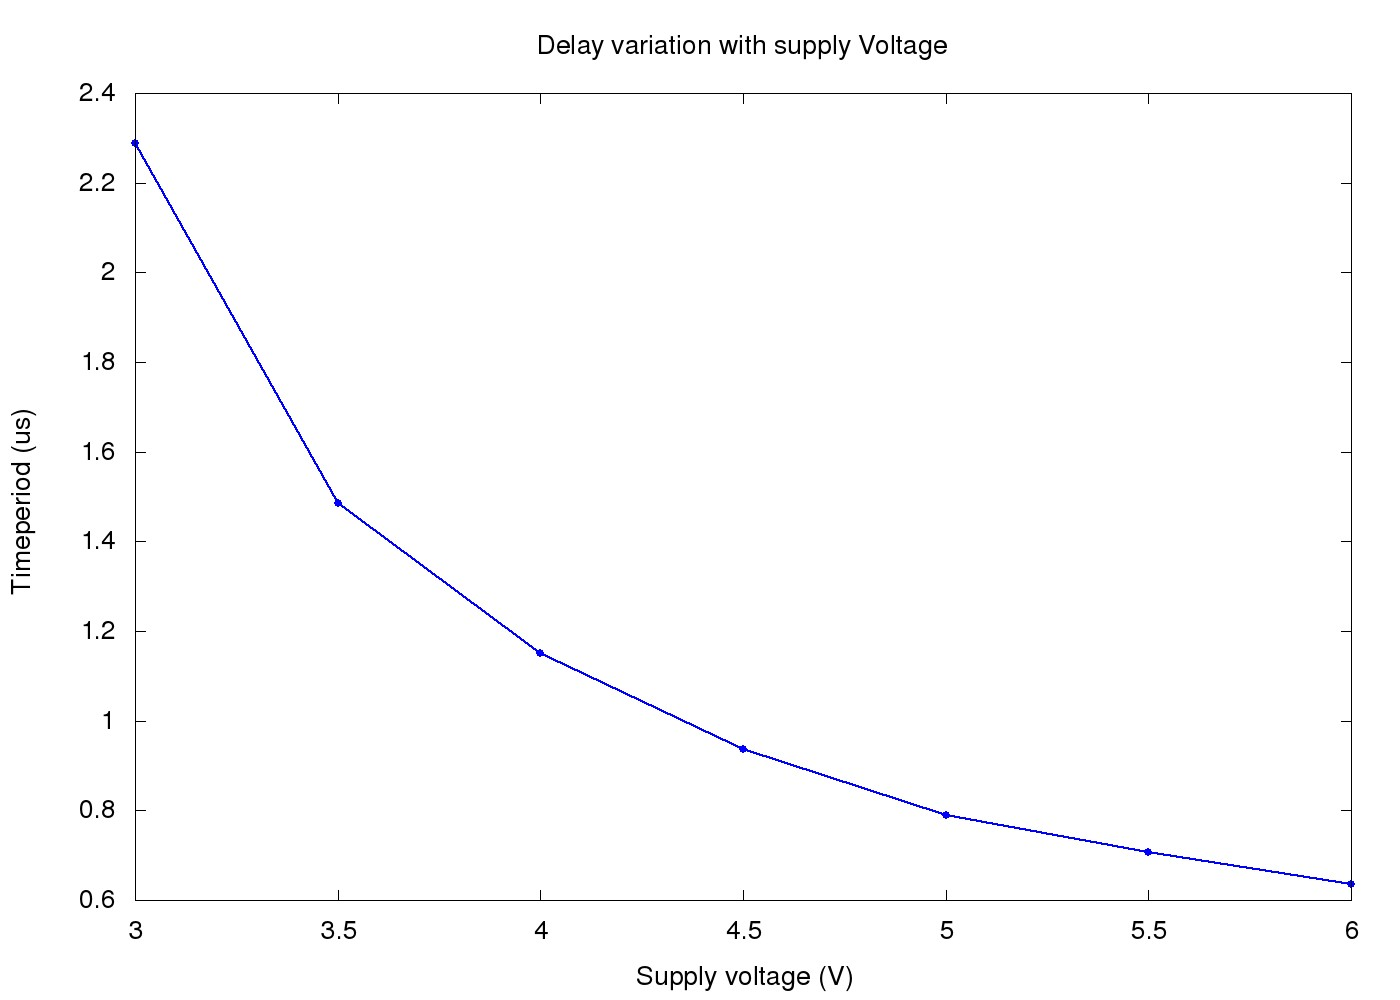
\includegraphics[scale=0.4]{figs/Supply_load_var.jpg}
    \caption{Delay variation with supply voltage}
    \label{fig:my_label}
\end{figure}
\vspace{15mm}
\subsection{Current drawn from the ring oscillator}
Whenever an inverter output switches from low to high, current is drawn
from the power supply. The current drawn is approximately a triangular
pulse whose width is essentially the delay of the gate. Therefore the current
drawn by each inverter in the ring oscillator is a triangular pulse train with
frequency equal to frequency of oscillation. The current drawn by the ring
oscillator is a summation of the individual currents drawn by the inverters
(note that the inverters switching events do not all happen at once). We
can connect a small resistor in series with ground path to observe this in
practice.
\begin{figure}
    \centering
    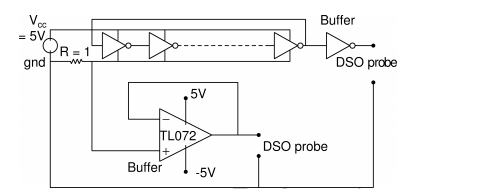
\includegraphics{figs/current.png}
    \caption{Setup to measure current}
    \label{fig:my_label}
\end{figure}

Peak current = \textbf{12 mA} , Average current drawn = \textbf{6.55 mA}

 
\end{document}
